\documentclass[10pt,twocolumn]{article}
\usepackage[a4paper,margin=0.75in,columnsep=0.25in]{geometry}
\usepackage[T1]{fontenc}
\usepackage{lmodern}
\usepackage{amsmath,amssymb}
\usepackage{graphicx}
\usepackage{booktabs}
\usepackage{multirow}
\usepackage{xcolor}
\usepackage{caption}
\usepackage{subcaption}
\usepackage{tikz}
\usetikzlibrary{arrows.meta,positioning,shapes.geometric}
\usepackage[hidelinks]{hyperref}
\usepackage{enumitem}
\setlist{nosep,leftmargin=*}
\captionsetup{font=small,labelfont=bf}

% ---- Leak-free segmentation retrain results (filled from results/clean_seg_results.json) ----
\newcommand{\bananaCleanMap}{82.1}
\newcommand{\bananaCleanMapNF}{46.6}
\newcommand{\mangoCleanMap}{94.6}
\newcommand{\mangoCleanMapNF}{71.1}

\title{\textbf{Pile-to-Score: Basket-Level Freshness Assessment of Market-Stall Produce via Decoupled Instance Segmentation and Crop-Level Ripeness Classification}}
\author{\textbf{Muhammad Abdul Wasay Abid}\\[2pt]
\small Faculty of Information Technology, University of Central Punjab, Lahore, Pakistan\\
\small \texttt{abdulwasayabid.801@gmail.com}\\
\small Code \& models: \url{https://github.com/WasayAbid/pile-to-score}}
\date{November 2026}
\raggedbottom

\begin{document}
\maketitle
\begin{abstract}
Image-based fruit freshness and ripeness classifiers are almost always trained and evaluated on photographs of a \emph{single} fruit against a clean background. Produce sold in informal street markets, however, is photographed as \emph{piles}: dozens of overlapping fruits in crates, baskets and carts, where a buyer or an online marketplace needs one trustworthy judgement for the whole lot. We present \textbf{Pile-to-Score}, a two-stage pipeline that converts a single market-stall photograph into a basket-level freshness score. Stage~1 is a class-agnostic YOLOv8m instance-segmentation model trained on stall photographs that isolates every visible fruit; Stage~2 classifies the ripeness of each crop with a fruit-specific classifier; a confidence-weighted aggregation rule with a spoilage penalty and explicit quality gating (``retake'' rules) produces a 0--100 score and a freshness tier. Because the two stages are decoupled, existing single-fruit ripeness datasets can be reused without re-annotating ripeness on pile images. We instantiate the pipeline for banana, mango, tomato and apple and deploy it behind a REST service integrated into a (pre-release) vendor-facing mobile marketplace application. Crop classifiers reach 98.6\% (banana, 6 classes), 92.0\% (mango, 4 classes) and 99.4\% (tomato, 4 classes) top-1 accuracy on held-out data, and the full pipeline processes a stall photograph containing 9--25 fruits in 0.4--1.1\,s on a desktop CPU. We additionally contribute a \emph{leakage audit}: a near-duplicate analysis reveals that the held-out segmentation splits of two of our four Roboflow-exported datasets are contaminated by training images, which would have inflated reported mask mAP; we quantify this effect, report classifier accuracy on de-duplicated subsets, and retrain the affected models on leak-free splits, which shows that the mango segmenter generalises (94.6\% mask mAP50) while the banana segmenter's reported 97\% falls to 82\%. Finally, we document a substantial domain gap between benchmark accuracy and behaviour on real stall crops, which we argue is the main open problem for this application.
\end{abstract}

\section{Introduction}
Post-harvest loss of fruit and vegetables is among the largest sources of food loss worldwide~\cite{fao2019}. In many low- and middle-income countries a large share of fresh produce is sold through informal channels---street carts, roadside stalls and wholesale \emph{mandis}---where quality is judged entirely by eye and there is no standard grading. As these vendors begin to sell through mobile marketplaces, customers lose even that visual inspection: they must trust a photograph and a vendor's description.

Computer vision is a natural fit for this problem, and deep-learning fruit classifiers are well studied~\cite{kamilaris2018,koirala2019}. However, the vast majority of freshness and ripeness work models a \emph{single} fruit per image~\cite{muresan2018,bird2022}, whereas detection and segmentation work in agriculture targets fruit \emph{on the tree} for yield estimation and robotic harvesting~\cite{sa2016,bargoti2017,liu2020yolotomato}. A vendor's photograph of a pile of bananas on a cart falls between these two bodies of work: it contains many fruits, heavy occlusion and cluttered backgrounds, and the desired output is not a per-fruit label but a single, honest summary of the lot.

A direct approach would be a single-stage detector whose classes are ripeness levels. That requires every fruit in every pile image to be annotated with \emph{both} a mask and a ripeness label---expensive, and ambiguous for small or occluded fruit. Instead we \emph{decouple} the problem:

\begin{enumerate}
  \item a class-agnostic segmentation model answers only ``where is each fruit?'', which is cheap to annotate on stall photographs; and
  \item a crop-level ripeness classifier answers ``how ripe is this fruit?'', for which public single-fruit datasets already exist.
\end{enumerate}

\noindent\textbf{Contributions.}
\begin{itemize}
  \item \textbf{Pile-to-Score}, a decoupled segmentation--classification pipeline that produces a basket-level freshness score from a single stall photograph, with a confidence-weighted aggregation rule, spoilage penalty, quality gating and multi-photograph fusion (Sec.~\ref{sec:method}).
  \item Four fruit-specific instantiations (banana, mango, tomato, apple), including class-agnostic \emph{stall-segmentation} datasets built from market photographs, and a production deployment in a mobile marketplace (Sec.~\ref{sec:data}, \ref{sec:deploy}).
  \item A reproducible \textbf{evaluation with a leakage audit}: we re-evaluate every model locally, detect near-duplicate contamination between training and held-out splits, report accuracy on de-duplicated subsets, and retrain affected segmentation models on leak-free splits (Sec.~\ref{sec:results}).
  \item An honest analysis of the \textbf{benchmark-to-stall domain gap}, showing that high in-distribution accuracy does not guarantee sensible behaviour on real stall crops (Sec.~\ref{sec:discussion}).
\end{itemize}

\section{Related Work}
\textbf{Single-item freshness and ripeness classification.} Convolutional networks pretrained on ImageNet~\cite{deng2009} and fine-tuned on fruit images routinely exceed 95\% accuracy on fresh/rotten or ripeness-stage classification~\cite{muresan2018,bird2022,kamilaris2018}. These datasets typically contain one fruit per image, centred and well lit, so they do not by themselves address pile images.

\textbf{Fruit detection and segmentation.} Region-based detectors and instance segmenters such as Mask R-CNN~\cite{he2017maskrcnn} and the YOLO family~\cite{redmon2016yolo,jocher2023yolov8} have been applied extensively to fruit in orchards and greenhouses~\cite{sa2016,bargoti2017,koirala2019}, sometimes with ripeness-aware classes, e.g.\ for tomatoes~\cite{liu2020yolotomato,laboro2020}. These systems target harvesting and yield rather than retail quality, and joint ripeness-and-mask labels must be collected for every training image.

\textbf{Foundation models.} Promptable segmenters such as SAM~\cite{kirillov2023sam} and multimodal models such as CLIP~\cite{radford2021clip} and Gemini~\cite{gemini2023} can, in principle, segment or describe produce zero-shot. They are, however, large, costly per request and not calibrated to a fixed ripeness taxonomy; our deployed system uses a multimodal LLM only as a fallback for produce types without a dedicated model.

\textbf{Data leakage in evaluation.} Overlap between training and test data is a well-documented source of over-optimistic results~\cite{kaufman2012leakage,kapoor2023leakage}; near-duplicate images are a particularly common form in vision benchmarks~\cite{barz2020}. Dataset tooling that augments images \emph{before} splitting, or that re-uses images across splits, can silently create such leakage. We audit for it explicitly.

\section{Method}\label{sec:method}

\begin{figure*}[t]
\centering
\resizebox{\textwidth}{!}{%
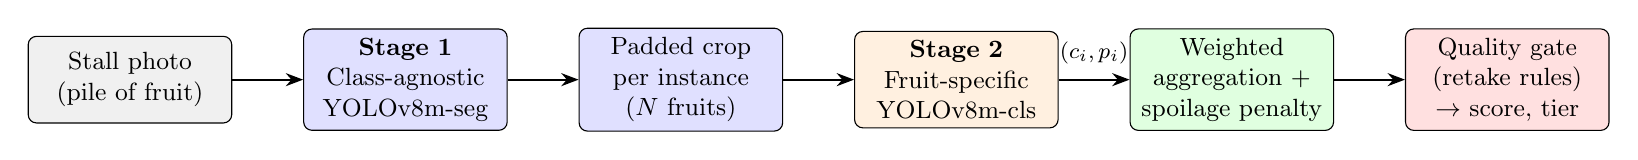
\begin{tikzpicture}[
  node distance=0.9cm,
  box/.style={draw, rounded corners=3pt, align=center, minimum height=1.1cm, text width=2.35cm, font=\small, fill=#1!12},
  box/.default=blue,
  arr/.style={-{Stealth[length=2.2mm]}, thick}]
\node[box=gray] (img) {Stall photo\\(pile of fruit)};
\node[box=blue, right=of img] (seg) {\textbf{Stage 1}\\Class-agnostic\\YOLOv8m-seg};
\node[box=blue, right=of seg] (crop) {Padded crop\\per instance\\($N$ fruits)};
\node[box=orange, right=of crop] (cls) {\textbf{Stage 2}\\Fruit-specific\\YOLOv8m-cls};
\node[box=green, right=of cls] (agg) {Weighted\\aggregation +\\spoilage penalty};
\node[box=red, right=of agg] (gate) {Quality gate\\(retake rules)\\$\rightarrow$ score, tier};
\draw[arr] (img) -- (seg); \draw[arr] (seg) -- (crop); \draw[arr] (crop) -- (cls);
\draw[arr] (cls) -- node[above=2pt,font=\footnotesize]{$(c_i,p_i)$} (agg); \draw[arr] (agg) -- (gate);
\end{tikzpicture}}
\caption{Pile-to-Score pipeline. Stage~1 locates every fruit without judging ripeness; Stage~2 classifies each crop; per-piece predictions $(c_i,p_i)$ are aggregated into a basket score $S\in[0,100]$ with a freshness tier, and low-quality inputs are rejected before a score is shown.}
\label{fig:pipeline}
\end{figure*}

\subsection{Stage 1: class-agnostic stall segmentation}
For each fruit type we train a single-class YOLOv8m-seg model~\cite{jocher2023yolov8} initialised from COCO~\cite{lin2014coco} weights. The model predicts an instance mask and box for every visible fruit, but \emph{not} its ripeness. Single-class training (\texttt{single\_cls}) concentrates model capacity on separating touching, overlapping fruit, which is the hard part of pile images, and makes annotation fast: annotators only outline fruit. Inference uses a low confidence threshold (0.10--0.20) to favour recall in dense piles. Each detection is expanded by 6\% of its box size on every side and cropped from the full-resolution image.

\subsection{Stage 2: crop-level ripeness classification}
Each crop is classified by a fruit-specific YOLOv8m-cls model (ImageNet-pretrained, $224\times224$ input). Class taxonomies follow the source datasets: six classes for banana (\emph{freshripe, freshunripe, ripe, unripe, overripe, rotten}), four for mango (\emph{unripe, partially ripe, ripe, overripe}), four for tomato (\emph{unripe, ripe, old, damaged}) and two for apple (\emph{fresh, rotten}). For mango, a lightweight HSV heuristic additionally flags large dark lesions, since the source taxonomy has no \emph{rotten} class.

\subsection{Basket-level aggregation}
Let a photograph contain $N$ segmented fruits with predicted classes $c_i$ and top-1 confidences $p_i$. Each class has a freshness weight $w(c)\in[0,1]$ reflecting saleability (e.g.\ ripe $=1.0$, partially ripe $=0.85$, unripe $=0.55$, overripe/rotten $=0.15$--$0.38$). The base score is the confidence-weighted mean
\begin{equation}
  B = \frac{100}{N}\sum_{i=1}^{N} w(c_i)\,p_i .
\end{equation}
Multiplying by $p_i$ means that uncertain predictions pull the score down rather than up, so the system errs towards caution. Because a few spoiled fruits matter more to a buyer than their arithmetic share, we subtract a step penalty based on the spoiled fraction $\rho = |\{i : c_i \in \mathcal{C}_{\text{spoil}}\}|/N$:
\begin{equation}
  S = \operatorname{clip}\big(B - \pi(\rho),\,0,\,100\big),
\end{equation}
where $\pi(\rho)\in\{0,5,10,20\}$ for thresholds $\rho\le 0.05, 0.15, 0.25, >0.25$ (banana uses a softer schedule $\{0,4,8,12\}$ at $0.10, 0.22, 0.35$, because its taxonomy already discounts overripe fruit). $S$ is mapped to five tiers: \emph{Premium Fresh} ($\ge 90$), \emph{Fresh} ($\ge 75$), \emph{Moderately Fresh} ($\ge 60$), \emph{Low Freshness} ($\ge 40$) and \emph{Poor Quality}.

\subsection{Quality gating and multi-photo fusion}
A score computed from a bad photograph is worse than no score. Before a score is published the pipeline therefore \emph{blocks} the result and asks for a retake if (i) no fruit is segmented, (ii) fewer than three fruits are segmented, or (iii) the mean classifier confidence is below 0.38; very low scores raise a \emph{warning} instead. Vendors may submit several photographs of the same lot; their results are fused by a piece-count-weighted mean, $S = \sum_k N_k S_k / \sum_k N_k$, with class histograms summed across photographs.

\subsection{Deployment}\label{sec:deploy}
The models are served by a FastAPI service exposing \texttt{/v1/freshness} (multipart image) and \texttt{/v1/freshness/url} (signed storage URL). In the vendor mobile application (React Native), a vendor photographs produce when listing it; a serverless function forwards the image to the service and stores the score, tier, class histogram and piece count with the listing. Vendors can rate each AI score from 1 to 5, creating a feedback channel for future human-aligned evaluation. Produce types without a dedicated model fall back to a multimodal LLM~\cite{gemini2023}.

\section{Datasets}\label{sec:data}
Table~\ref{tab:data} summarises the data. Stage~1 datasets were built by the author from market and stall photographs collected from the web and from approximately 30 photographs taken by the author, annotated with instance masks on Roboflow and exported with Roboflow augmentation. Stage~2 datasets are public single-fruit datasets, re-split where noted.

\begin{table}[t]
\centering\small
\caption{Datasets. Images are listed as train/val/test. Stage~1 counts are after Roboflow augmentation; ``src'' gives unique source photographs in the training split.}
\label{tab:data}
\setlength{\tabcolsep}{3pt}
\resizebox{\columnwidth}{!}{%
\begin{tabular}{@{}llll@{}}
\toprule
Fruit & Stage & Source & Images \\
\midrule
Banana & 1 seg & own (stall) & 112/22/11 \\
       & 2 cls & Roboflow c3a2v~\cite{rf_banana} & 3931/1123/562 \\
Mango  & 1 seg & own (stall) & 264/11/11 (88 src) \\
       & 2 cls & Roboflow cadimedia~\cite{rf_mango} & 1597/200/199 \\
Tomato & 1 seg & own (stall) & 210/31/18 (69 src) \\
       & 2 cls & VegNet (Kaggle)~\cite{vegnet} & 6501/725/-- \\
Apple  & 1 seg & own (stall) & 176/21/13 (59 src)$^\ast$ \\
       & 2 cls & public fresh/rotten~\cite{rf_apple} & 1406/401/199 \\
\bottomrule
\end{tabular}}
\par\vspace{3pt}
{\footnotesize\raggedright $^\ast$ Locally archived export; the training run logged 204/21/16.\par}
\end{table}

For mango, the original \emph{Early Ripe} and \emph{Partially Ripe} classes were merged into \emph{partially ripe}, and the pooled data were re-split with stratified 80/10/10 sampling. The tomato dataset provides only train and validation splits; we therefore report tomato classifier results on the validation split and treat them as optimistic, since that split was also used for checkpoint selection.

\section{Experimental Setup}
\textbf{Training.} All models were trained in Google Colab with Ultralytics~8.4~\cite{jocher2023yolov8}. Segmentation models and the mango classifier used a two-phase schedule: (1) a frozen backbone for 25 epochs (\texttt{freeze}=10 for segmentation, 8 for classification) to adapt the head, and (2) full fine-tuning with a lower learning rate (AdamW~\cite{loshchilov2019adamw}, $\text{lr}_0 = 2\!\times\!10^{-4}$--$3\!\times\!10^{-4}$) and early stopping. Segmentation used $640\times640$ inputs with mosaic disabled, since mosaic tiles break the spatial context of piles. The mango classifier was regularised with dropout 0.25, mixup 0.10~\cite{zhang2018mixup}, label smoothing 0.10~\cite{szegedy2016} and weight decay $10^{-3}$, given its small training set.

\textbf{Evaluation.} All numbers in Sec.~\ref{sec:results} were \emph{re-computed locally} from the released weights on an AMD Ryzen~5 7500F CPU (16\,GB RAM). We report top-1 accuracy, macro precision, recall and F1 for classifiers, and mask/box mAP@0.5 and mAP@0.5:0.95 for segmentation.

\textbf{Leakage audit.} For every held-out image we compute the maximum normalised cross-correlation (NCC) between its $32\times32$ grayscale thumbnail (and its horizontal flip) and every training thumbnail ($24\times24$ for the larger classification sets). As a control, NCC between unrelated images from \emph{different} fruit datasets lies between 0.19 and 0.52. We treat NCC $\ge 0.95$ as a near-duplicate; at the segmentation scale we also inspect pairs with NCC $\ge 0.85$, which correspond to augmented copies (crops, colour shifts) of the same source photograph.

\section{Results}\label{sec:results}

\subsection{Crop-level ripeness classification}
Table~\ref{tab:cls} and Fig.~\ref{fig:cm} report classifier performance. Banana and tomato classifiers are near-saturated. Mango is the hardest task (92.0\%): errors concentrate between \emph{partially ripe} and its neighbours \emph{ripe} and \emph{unripe} (Fig.~\ref{fig:cm}b), which is expected for an ordinal, visually continuous property. Top-2 accuracy is $\ge 99.5\%$ for all three fruits, so nearly every error is between adjacent stages. CPU latency is about 32\,ms per crop. The apple classifier reached 100\% top-1 on its validation split in training; since that dataset is not available for independent re-evaluation and a perfect score on a public fresh/rotten set is itself a warning sign of near-duplicates, we do not report it as a result.

\begin{table}[t]
\centering\small
\caption{Crop classifier results, re-computed locally on held-out data.}
\label{tab:cls}
\setlength{\tabcolsep}{3.5pt}
\resizebox{\columnwidth}{!}{%
\begin{tabular}{@{}lcccccc@{}}
\toprule
Fruit & Split & $n$ & Top-1 & Top-2 & Macro-F1 & ms/crop \\
\midrule
Banana (6) & test & 562 & 98.6 & 100.0 & 97.8 & 31.4 \\
Mango (4)  & test & 199 & 92.0 & 99.5  & 91.5 & 31.8 \\
Tomato (4) & val  & 724 & 99.4 & 100.0 & 99.4 & 33.2 \\
\bottomrule
\end{tabular}}
\end{table}

\begin{figure*}[t]
\centering
\begin{subfigure}{0.36\textwidth}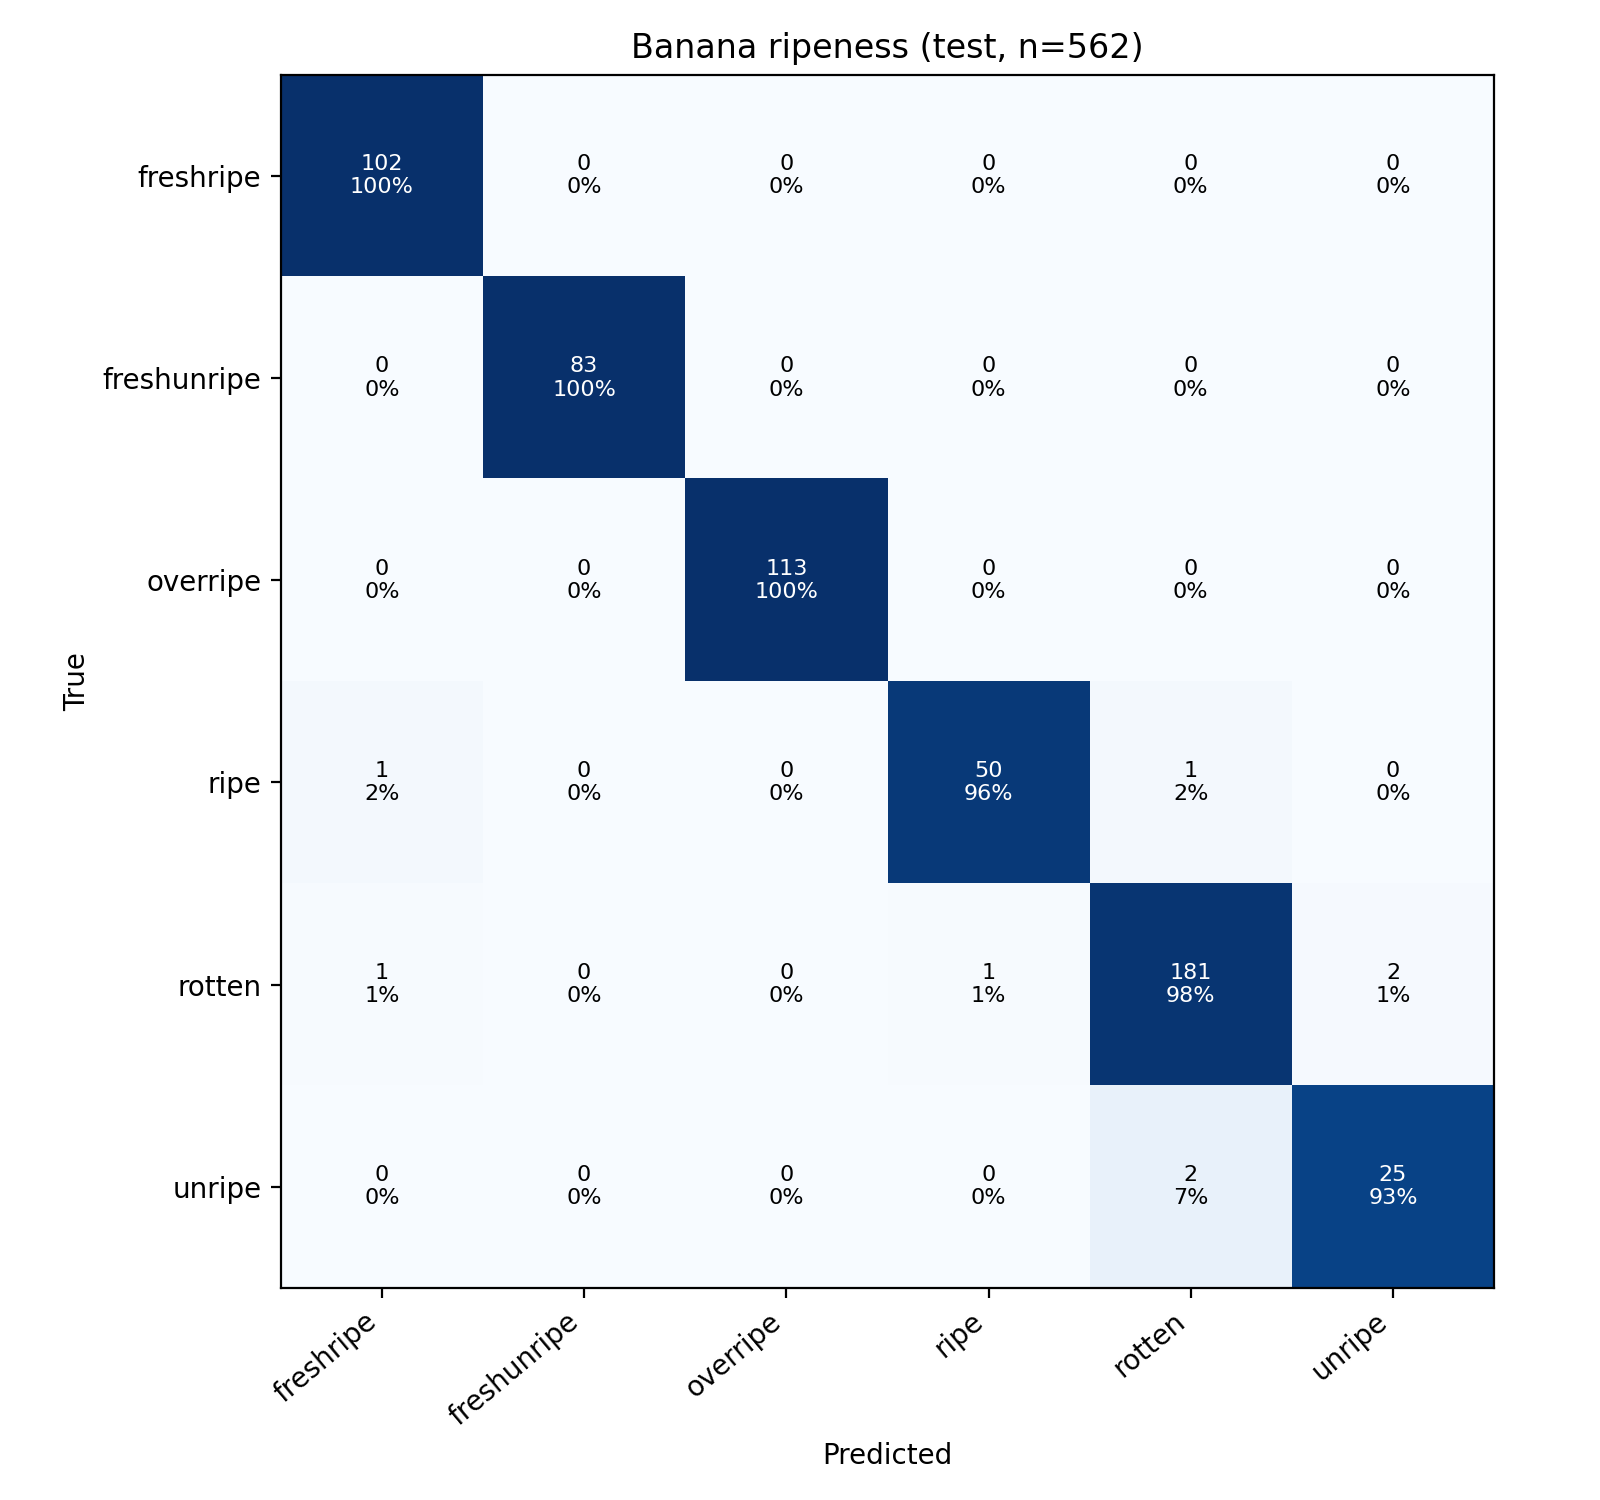
\includegraphics[width=\linewidth]{figures/cm_banana.png}\caption{Banana (test)}\end{subfigure}\hfill
\begin{subfigure}{0.3\textwidth}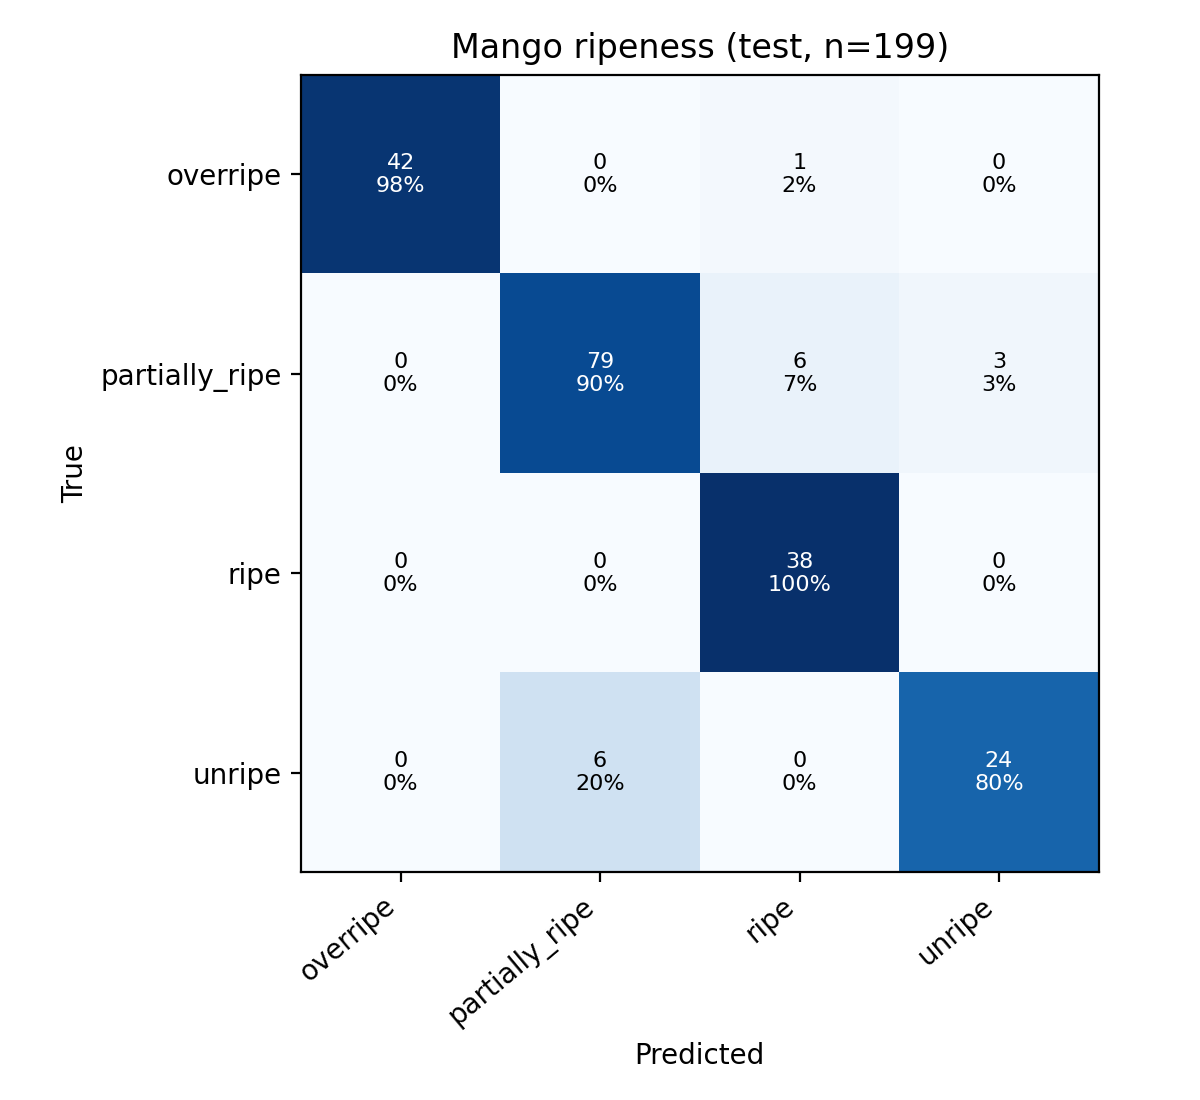
\includegraphics[width=\linewidth]{figures/cm_mango.png}\caption{Mango (test)}\end{subfigure}\hfill
\begin{subfigure}{0.3\textwidth}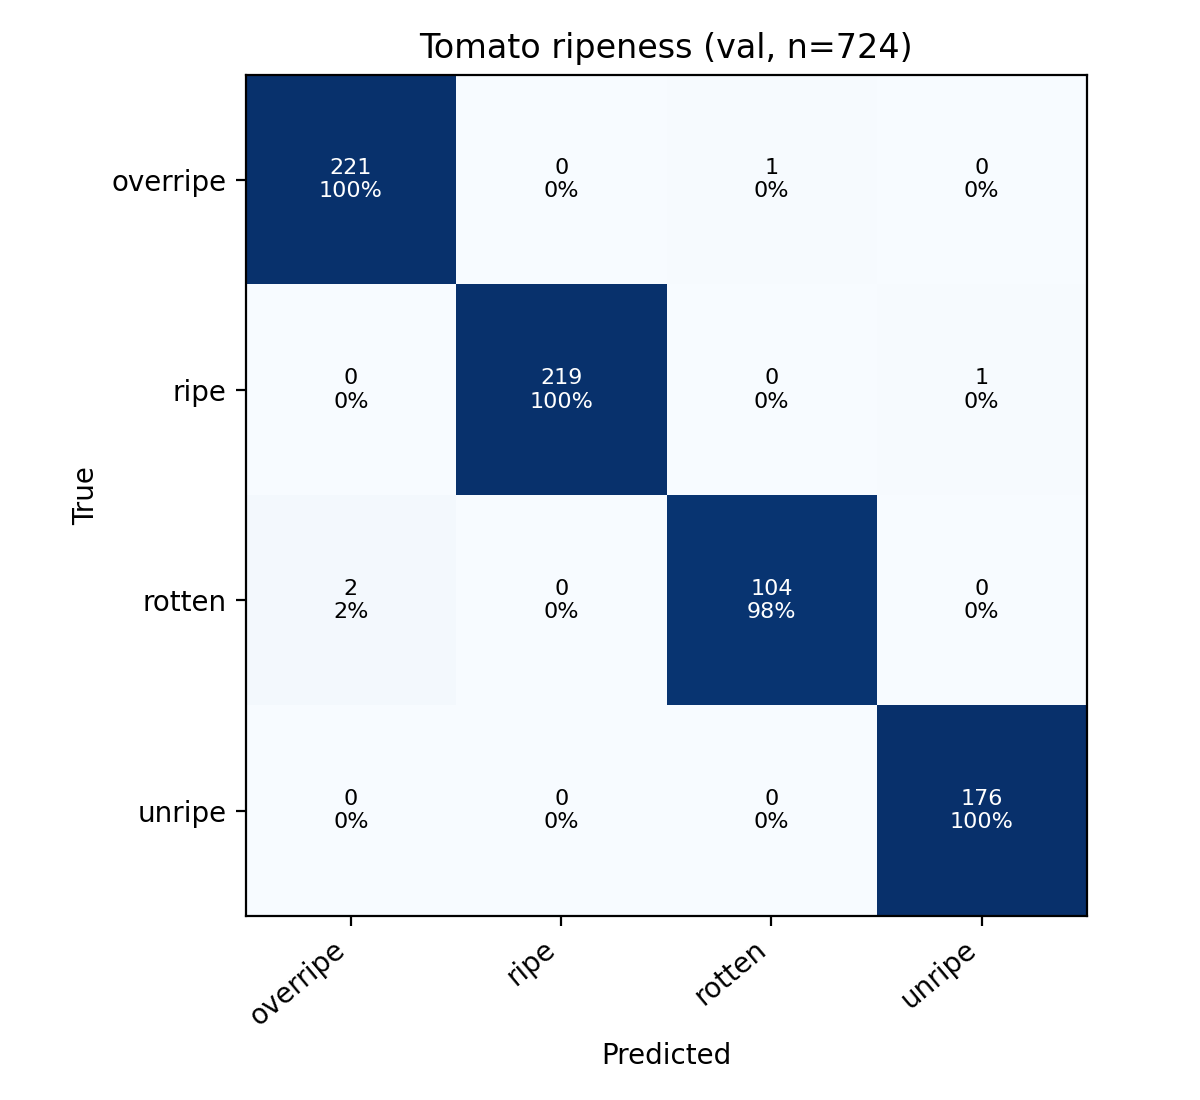
\includegraphics[width=\linewidth]{figures/cm_tomato.png}\caption{Tomato (val)}\end{subfigure}
\caption{Confusion matrices of the crop ripeness classifiers (counts and row-normalised percentages). Tomato classes \emph{overripe} and \emph{rotten} correspond to the dataset's \emph{old} and \emph{damaged}.}
\label{fig:cm}
\end{figure*}

\textbf{Robustness to near-duplicates.} The audit (Table~\ref{tab:leak_cls}) shows that 55\% of banana test images and 26\% of tomato validation images have a near-duplicate (NCC $\ge 0.95$) in the training split, while the re-split mango test set has none. Restricting evaluation to images \emph{without} a near-duplicate changes accuracy by at most 1 percentage point, so the classifiers' performance is not an artefact of memorisation.

\begin{table}[t]
\centering\small
\caption{Classifier accuracy on all held-out images vs.\ only those without a near-duplicate in training (NCC $< 0.95$).}
\label{tab:leak_cls}
\begin{tabular}{@{}lcccc@{}}
\toprule
 & \multicolumn{2}{c}{All held-out} & \multicolumn{2}{c}{De-duplicated} \\
\cmidrule(lr){2-3}\cmidrule(lr){4-5}
Fruit & $n$ & Top-1 & $n$ & Top-1 \\
\midrule
Banana & 562 & 98.6 & 253 & 97.6 \\
Mango  & 199 & 92.0 & 199 & 92.0 \\
Tomato & 724 & 99.4 & 533 & 99.4 \\
\bottomrule
\end{tabular}
\end{table}

\subsection{Stall segmentation and the leakage audit}
Table~\ref{tab:seg} compares the test metrics logged during training with our local re-evaluation and the leakage audit. Local re-evaluation reproduces the logged numbers to within about 1 point. The audit, however, shows that \textbf{all 11 banana test images are pixel-identical} (NCC $=1.00$) to training images, and so are all 22 banana validation images: the Roboflow export placed the held-out images in the training split as well. For mango, 10 of 11 test images have NCC $\ge 0.90$ with a training image (control: $\le 0.52$). These are augmented copies of the same source photographs, a consequence of augmenting before splitting. The apple test split is clean (max NCC 0.49, in the range of the cross-fruit control). The banana and mango test metrics therefore measure memorisation as much as generalisation.

To obtain honest estimates we removed every training image with NCC $\ge 0.85$ to any validation or test image (banana: 36 of 112 removed; mango: 151 of 264 removed), retrained both models with the same two-phase recipe (15 frozen + up to 60 fine-tuning epochs, on a local GTX~1660~Ti), and evaluated on the untouched test split. The resulting \emph{leak-free} numbers are in the last column of Table~\ref{tab:seg}. They are trained on substantially less data, so they are a \emph{lower bound} on what the full-data model would achieve on genuinely unseen photographs. The two fruits behave very differently. Mango is unaffected (94.6\% leak-free vs.\ 94.2\% re-evaluated), so its segmenter generalises to unseen stall photographs despite losing 57\% of its training images. Banana drops from 97.3\% to 82.1\% mask mAP50 and from 71.9\% to 46.6\% mAP50:95: roughly 15 points of the originally reported score reflected memorised test images, and boundary quality on tightly packed banana hands is the weakest part of the system. Without the audit, the banana segmenter would have looked like the strongest model rather than the weakest. On a GTX~1660~Ti, segmentation inference takes about 27--28\,ms per image.

\begin{table*}[t]
\centering\small
\caption{Stage-1 stall segmentation, test split. ``Logged'': reported at training time. ``Re-eval.'': our local re-evaluation of the released weights. ``Dup.'': test images with a near-duplicate in the training split. ``Leak-free'': model retrained after removing near-duplicates of held-out images from training. All values are mask mAP (\%).}
\label{tab:seg}
\resizebox{\textwidth}{!}{%
\begin{tabular}{@{}lccccccc@{}}
\toprule
 & Test images / & Logged & \multicolumn{2}{c}{Re-evaluated} & Test near- & \multicolumn{2}{c}{Leak-free retrain} \\
\cmidrule(lr){4-5}\cmidrule(lr){7-8}
Fruit & instances & mAP50 & mAP50 & mAP50:95 & duplicates & mAP50 & mAP50:95 \\
\midrule
Banana & 11 / 622  & 96.3 & 97.3 & 71.9 & 11/11 & \textbf{\bananaCleanMap} & \textbf{\bananaCleanMapNF} \\
Mango  & 11 / 244  & 93.2 & 94.2 & 75.2 & 10/11 & \textbf{\mangoCleanMap} & \textbf{\mangoCleanMapNF} \\
Apple  & 13 / 821  & 80.3 & 80.4 & 59.7 & 0/13  & 80.4$^\ast$ & 59.7$^\ast$ \\
Tomato & 18 / 1286 & 87.5 & n/a$^\dagger$ & n/a$^\dagger$ & -- & -- & -- \\
\bottomrule
\end{tabular}}
\par\vspace{3pt}
{\footnotesize\raggedright $^\ast$ Apple test split is already clean; no retraining needed. \quad $^\dagger$ The exact v4 tomato export used for training was not archived locally, so it could not be re-evaluated; the logged value is reported for completeness only.\par}
\end{table*}

\subsection{End-to-end pipeline on stall photographs}
We ran the full pipeline on 25 vendor-style stall photographs per fruit (14 for apple) collected from the web, none of which carry ripeness ground truth. Some of these photographs are also sources of the Stage-1 training data, so we use them only to characterise throughput and gating behaviour, not accuracy. Table~\ref{tab:e2e} reports throughput and gating behaviour, and Fig.~\ref{fig:qual} shows examples. On a desktop CPU a full photograph is processed in 0.4--1.1\,s, dominated by the segmenter ($\approx$300\,ms) and $N$ crop classifications ($\approx$32\,ms each), which is acceptable for an interactive listing flow without a GPU.

\begin{table}[t]
\centering\small
\caption{End-to-end behaviour on unlabelled stall photographs (CPU).}
\label{tab:e2e}
\setlength{\tabcolsep}{4pt}
\resizebox{\columnwidth}{!}{%
\begin{tabular}{@{}lcccc@{}}
\toprule
Fruit & Photos & Fruits / photo & ms / photo & Retakes \\
\midrule
Banana & 25 & 21.0 & 811  & 8 \\
Mango  & 25 & 20.0 & 810  & 1 \\
Tomato & 25 & 8.9  & 429  & 16 \\
Apple  & 14 & 24.7 & 1064 & 0 \\
\bottomrule
\end{tabular}}
\end{table}

\begin{figure*}[t]
\centering
\resizebox{\textwidth}{!}{%
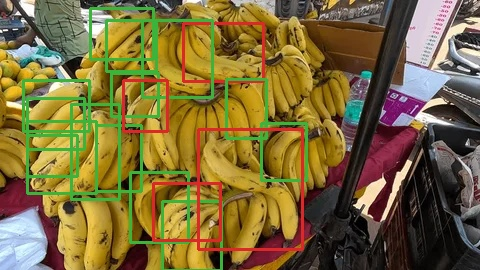
\includegraphics[height=4cm]{figures/banana_2.jpg}\hspace{4pt}%
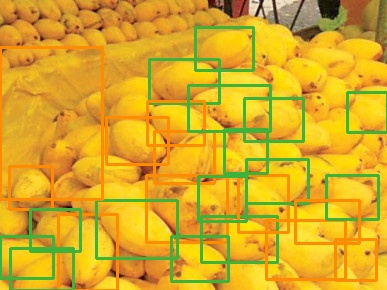
\includegraphics[height=4cm]{figures/mango_2.jpg}\hspace{4pt}%
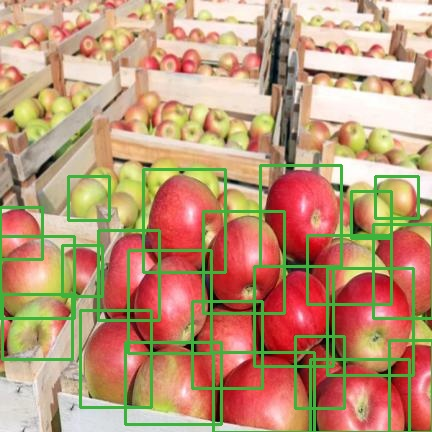
\includegraphics[height=4cm]{figures/apple_2.jpg}\hspace{4pt}%
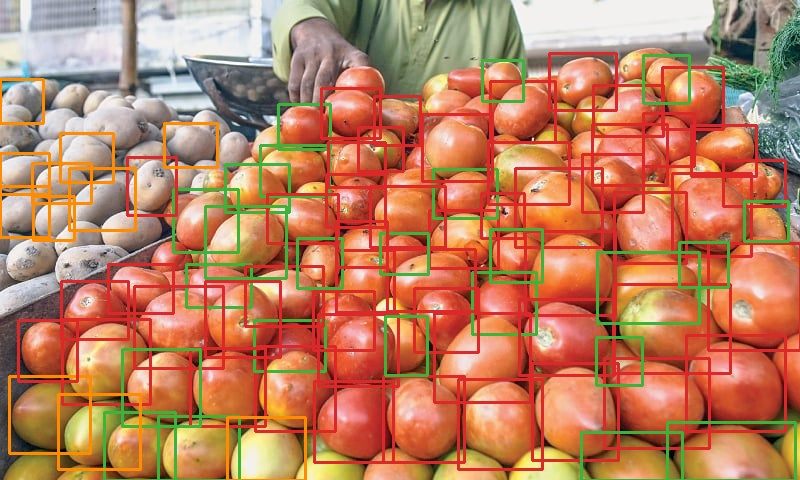
\includegraphics[height=4cm]{figures/tomato_2.jpg}}
\caption{Pipeline output on stall photographs (left to right: banana, mango, apple, tomato). Each box is one Stage-1 instance, coloured by its Stage-2 class: green = ripe/fresh, orange = unripe/partially ripe, red = overripe/rotten/damaged. The tomato example shows two failure modes discussed in Sec.~\ref{sec:discussion}: potatoes at the left are segmented as tomatoes, and many visually ripe tomatoes are classified as \emph{damaged}.}
\label{fig:qual}
\end{figure*}

\section{Discussion}\label{sec:discussion}
\textbf{Why decoupling helps.} Separating ``where'' from ``how ripe'' let us build pile-level systems for four fruits with only a few hundred segmentation images per fruit and no ripeness annotation on pile images. Either stage can be upgraded independently: a better public ripeness dataset improves Stage~2 without touching Stage~1. The class-agnostic segmenter is also robust to taxonomy changes; tomato and mango classifiers with different class sets plug into the same aggregation code.

\textbf{Benchmark accuracy is not stall accuracy.} The tomato classifier scores 99.4\% on its benchmark, yet on real stall crops it labels many visibly ripe tomatoes as \emph{damaged}, and 16 of 25 tomato stall photographs were rejected by the quality gate (Table~\ref{tab:e2e}, Fig.~\ref{fig:qual}). Benchmark images are close-ups under controlled lighting; stall crops are small, partly occluded, motion-blurred and lit by sunlight or coloured shade cloth. Conversely, the apple pipeline assigns a perfect score to almost every photograph, which suggests that a binary fresh/rotten taxonomy is too coarse for retail grading. In both cases the quality gate behaves as intended, refusing a score rather than publishing a misleading one, but closing the domain gap requires ripeness labels on \emph{stall crops}, which Stage~1 now makes cheap to generate.

\textbf{Leakage is easy to miss.} Two of our four segmentation datasets had contaminated test splits, even though the training logs looked normal. The cause was routine tooling behaviour: augmenting before splitting, and an export that placed held-out images in the training split. We recommend that any work reporting metrics on Roboflow-style exports run a near-duplicate audit like ours; it takes minutes on a CPU.

\textbf{Limitations.} (i) We have no basket-level ground truth, so the aggregation rule and its class weights are hand-designed and not yet validated against human graders; the vendor rating channel in the deployed app is intended to collect this. (ii) Segmentation test sets are small (11--18 images, though hundreds of instances). (iii) The tomato classifier is evaluated on a validation split also used for model selection. (iv) Stall photographs are mostly web-sourced and may not represent every market or camera.

\section{Conclusion}
We presented Pile-to-Score, a decoupled segmentation--classification pipeline that turns one photograph of a market-stall pile into a basket-level freshness score, instantiated for four fruits and deployed in a vendor marketplace application. Crop classifiers achieve 92--99\% held-out accuracy, robust to near-duplicate removal, and the full pipeline runs in about one second on a CPU. A leakage audit uncovered contaminated segmentation test splits. Retraining on leak-free splits confirmed the mango segmenter (94.6\% mask mAP50) but revised the banana segmenter from 97\% to 82\%, showing why such audits should be routine. Future work will (1) collect human basket-level freshness ratings to calibrate and validate the aggregation rule, (2) label stall crops produced by Stage~1 to close the domain gap, and (3) compare the pipeline against zero-shot multimodal models on the same basket-level benchmark.

\section*{Data and Code Availability}
All trained model weights (including the leak-free retrained segmenters), the inference pipeline, evaluation scripts and per-model metrics are publicly available at \url{https://github.com/WasayAbid/pile-to-score}.

\section*{Acknowledgements}
The author thanks the Faculty of Information Technology, University of Central Punjab, and the project lead for guidance during development.

\small
\begin{thebibliography}{99}
\bibitem{fao2019} FAO. \emph{The State of Food and Agriculture 2019: Moving Forward on Food Loss and Waste Reduction}. Food and Agriculture Organization of the United Nations, Rome, 2019.
\bibitem{kamilaris2018} A.~Kamilaris and F.~X. Prenafeta-Bold\'u. Deep learning in agriculture: A survey. \emph{Computers and Electronics in Agriculture}, 147:70--90, 2018.
\bibitem{koirala2019} A.~Koirala, K.~B. Walsh, Z.~Wang, and C.~McCarthy. Deep learning -- Method overview and review of use for fruit detection and yield estimation. \emph{Computers and Electronics in Agriculture}, 162:219--234, 2019.
\bibitem{muresan2018} H.~Mure\c{s}an and M.~Oltean. Fruit recognition from images using deep learning. \emph{Acta Universitatis Sapientiae, Informatica}, 10(1):26--42, 2018.
\bibitem{bird2022} J.~J. Bird, C.~M. Barnes, L.~J. Manso, A.~Ek\'art, and D.~R. Faria. Fruit quality and defect image classification with conditional GAN data augmentation. \emph{Scientia Horticulturae}, 293:110684, 2022.
\bibitem{sa2016} I.~Sa, Z.~Ge, F.~Dayoub, B.~Upcroft, T.~Perez, and C.~McCool. DeepFruits: A fruit detection system using deep neural networks. \emph{Sensors}, 16(8):1222, 2016.
\bibitem{bargoti2017} S.~Bargoti and J.~Underwood. Deep fruit detection in orchards. In \emph{IEEE International Conference on Robotics and Automation (ICRA)}, 2017.
\bibitem{liu2020yolotomato} G.~Liu, J.~C. Nouaze, P.~L. Touko~Mbouembe, and J.~H. Kim. YOLO-Tomato: A robust algorithm for tomato detection based on YOLOv3. \emph{Sensors}, 20(7):2145, 2020.
\bibitem{laboro2020} Laboro.AI. Laboro Tomato: Instance segmentation dataset. \url{https://github.com/laboroai/LaboroTomato}, 2020.
\bibitem{he2017maskrcnn} K.~He, G.~Gkioxari, P.~Doll\'ar, and R.~Girshick. Mask R-CNN. In \emph{IEEE International Conference on Computer Vision (ICCV)}, 2017.
\bibitem{redmon2016yolo} J.~Redmon, S.~Divvala, R.~Girshick, and A.~Farhadi. You only look once: Unified, real-time object detection. In \emph{IEEE/CVF Conference on Computer Vision and Pattern Recognition (CVPR)}, 2016.
\bibitem{jocher2023yolov8} G.~Jocher, A.~Chaurasia, and J.~Qiu. Ultralytics YOLOv8. \url{https://github.com/ultralytics/ultralytics}, 2023.
\bibitem{lin2014coco} T.-Y. Lin, M.~Maire, S.~Belongie, et~al. Microsoft COCO: Common objects in context. In \emph{European Conference on Computer Vision (ECCV)}, 2014.
\bibitem{deng2009} J.~Deng, W.~Dong, R.~Socher, L.-J. Li, K.~Li, and L.~Fei-Fei. ImageNet: A large-scale hierarchical image database. In \emph{CVPR}, 2009.
\bibitem{kirillov2023sam} A.~Kirillov, E.~Mintun, N.~Ravi, et~al. Segment anything. In \emph{ICCV}, 2023.
\bibitem{radford2021clip} A.~Radford, J.~W. Kim, C.~Hallacy, et~al. Learning transferable visual models from natural language supervision. In \emph{International Conference on Machine Learning (ICML)}, 2021.
\bibitem{gemini2023} Gemini Team, Google. Gemini: A family of highly capable multimodal models. \emph{arXiv:2312.11805}, 2023.
\bibitem{kaufman2012leakage} S.~Kaufman, S.~Rosset, C.~Perlich, and O.~Stitelman. Leakage in data mining: Formulation, detection, and avoidance. \emph{ACM Transactions on Knowledge Discovery from Data}, 6(4):15, 2012.
\bibitem{kapoor2023leakage} S.~Kapoor and A.~Narayanan. Leakage and the reproducibility crisis in machine-learning-based science. \emph{Patterns}, 4(9):100804, 2023.
\bibitem{barz2020} B.~Barz and J.~Denzler. Do we train on test data? Purging CIFAR of near-duplicates. \emph{Journal of Imaging}, 6(6):41, 2020.
\bibitem{loshchilov2019adamw} I.~Loshchilov and F.~Hutter. Decoupled weight decay regularization. In \emph{International Conference on Learning Representations (ICLR)}, 2019.
\bibitem{zhang2018mixup} H.~Zhang, M.~Cisse, Y.~N. Dauphin, and D.~Lopez-Paz. mixup: Beyond empirical risk minimization. In \emph{ICLR}, 2018.
\bibitem{szegedy2016} C.~Szegedy, V.~Vanhoucke, S.~Ioffe, J.~Shlens, and Z.~Wojna. Rethinking the Inception architecture for computer vision. In \emph{CVPR}, 2016.
\bibitem{rf_banana} Mahasarakham University. Banana ripeness classification dataset (banana-ripeness-c3a2v). Roboflow Universe. \url{https://universe.roboflow.com/mahasarakham-university-yeff9/banana-ripeness-c3a2v}.
\bibitem{rf_mango} cadimedia. MangoRipenessDetection dataset. Roboflow Universe. \url{https://universe.roboflow.com/cadimedia/mangoripenessdetection}.
\bibitem{vegnet} VegNet: vegetable quality image dataset (tomato subset: Unripe, Ripe, Old, Damaged). Kaggle.
\bibitem{rf_apple} Apple freshness (fresh/rotten) image dataset. Roboflow Universe.
\end{thebibliography}
\end{document}
